% *********************************************************************
% © 2021–2024 Jeremy Sylvestre
%
% Permission is granted to copy, distribute and/or modify this document
% under the terms of the GNU Free Documentation License, Version 1.3 or
% any later version published by the Free Software Foundation; with no
% Invariant Sections, no Front-Cover Texts, and no Back-Cover Texts. A
% copy of the license is included in the appendix entitled “GNU Free
% Documentation License” that appears in the output document of this
% PreTeXt source code. All trademarks™ are the registered® marks of
% their respective owners.
%
% *********************************************************************

\newcommand*{\xmin}{-0.5}
\newcommand*{\xmax}{3.25}
\newcommand*{\ymin}{-0.5}
\newcommand*{\ymax}{10}

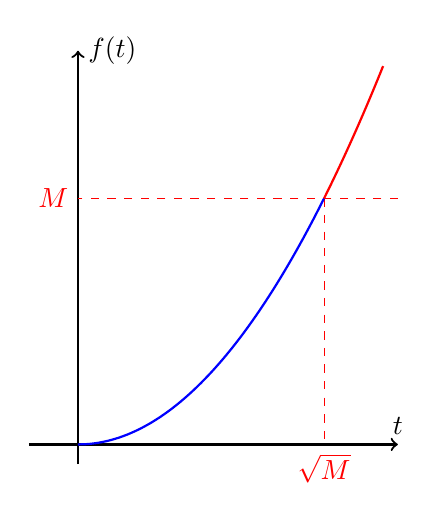
\begin{tikzpicture}
[
	closedpt/.style={circle,draw,fill,inner sep=0pt,minimum size=4pt},
	openpt/.style={circle,draw,inner sep=0pt,minimum size=4pt},
	yscale=0.5,
	xscale=1.25
]

	% axes
	\draw[->,thick] (\xmin,0) -- (\xmax,0) node[above] {$t$};
	\draw[->,thick] (0,\ymin) -- (0,\ymax) node[right] {$f(t)$};

	% graph
	\draw[dashed,red] (\xmax,6.25) -- (0,6.25) node[left] {$M$};
	\draw[dashed,red] (2.5,6.25) -- (2.5,0) node[below] {$\sqrt{M}$};
	\draw[thick, blue, domain=0:2.5, smooth] plot (\x,{\x * \x});
	\draw[thick, red, domain=2.5:3.1, smooth] plot (\x,{\x * \x});

\end{tikzpicture}
